\scanpage{35}
\mspage{34}
% Reused typed sheet, read after rotation through 180 degrees.
\begin{center}-3.11-\end{center}
Moreover, the section:
\[
(D_{\alpha_0,\ldots\alpha_n})^{n+1}\in\Gamma(\mathcal U_{\mathrm{reg}},L_{\alpha_0}^{n+1}\otimes\cdots\otimes L_{\alpha_n}^{n+1})
\]
is invariant in the $\mathrm{SL}(n+1)$-linearization of this sheaf, hence in the $\mathrm{PGL}(n)$-linearization of this sheaf, . Therefore, according to SGA 8, \S1, there is a section $E_{\alpha_0,\ldots\alpha_n}$ of $M_{\alpha_0}\otimes\cdots\otimes M_{\alpha_n}$ such that:
\[
(D_{\alpha_0,\ldots\alpha_n})^{n+1}=\unsure{\Phi|\bar\Phi}^{*}(E_{\alpha_0,\ldots\alpha_n}).
\]
\figure{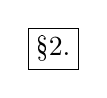
\begin{tikzpicture}[baseline=(heading.base)]\node[draw,inner sep=3pt] (heading) {\S2.};\end{tikzpicture}} The purpose of this section is to show that although $M_0\otimes\cdots\otimes M_m$ is not ample on $Z$ - which is not even a scheme - it is ample on a fairly large open subset $Z_0\subset Z$. We first define the subset $\unsure{\Phi|\bar\Phi}^{-1}(Z_0)$ of $\mathcal U_{\mathrm{reg}}$:

\uline{Definition 3.7}/\uline{Proposition 3.4}: $\mathcal U_{\mathrm{stable}}$ is the open subset of $(\mathbb P_n)^{m+1}$ whose geometric points $x=(x^{(0)},\ldots,x^{(m)})$ are those points such that for every proper linear subspace $L\subset\overline{\mathbb P}_n$:
\[
\frac{\text{number of points }x^{(i)}\text{ in }L}{m+1}<\frac{\dim L+1}{n+1}.
\]
\uline{Proof}: Consider the set of all pairs $\{I,n_0\}$ consisting of a subset $I\subset\{0,1,\ldots,m\}$ and an integer $n_0$ between 0 and $n-1$ such that:
\[
\frac{\text{cardinality of }I}{m+1}\geq\frac{n_0+1}{n+1}.
\]
Then the set of geometric points \uline{not} satisfying the above condition is the (finite) union over all $\{I,n_0\}$ of the sets consisting of
